\documentclass{standalone}
\usepackage{tkz-fct}
\usepackage{tkz-euclide}
\usepackage{color}
\renewcommand*\familydefault{\sfdefault}
\usepackage{sansmath}
\sansmath
\definecolor{gray75}{gray}{0.75}
\begin{document}
 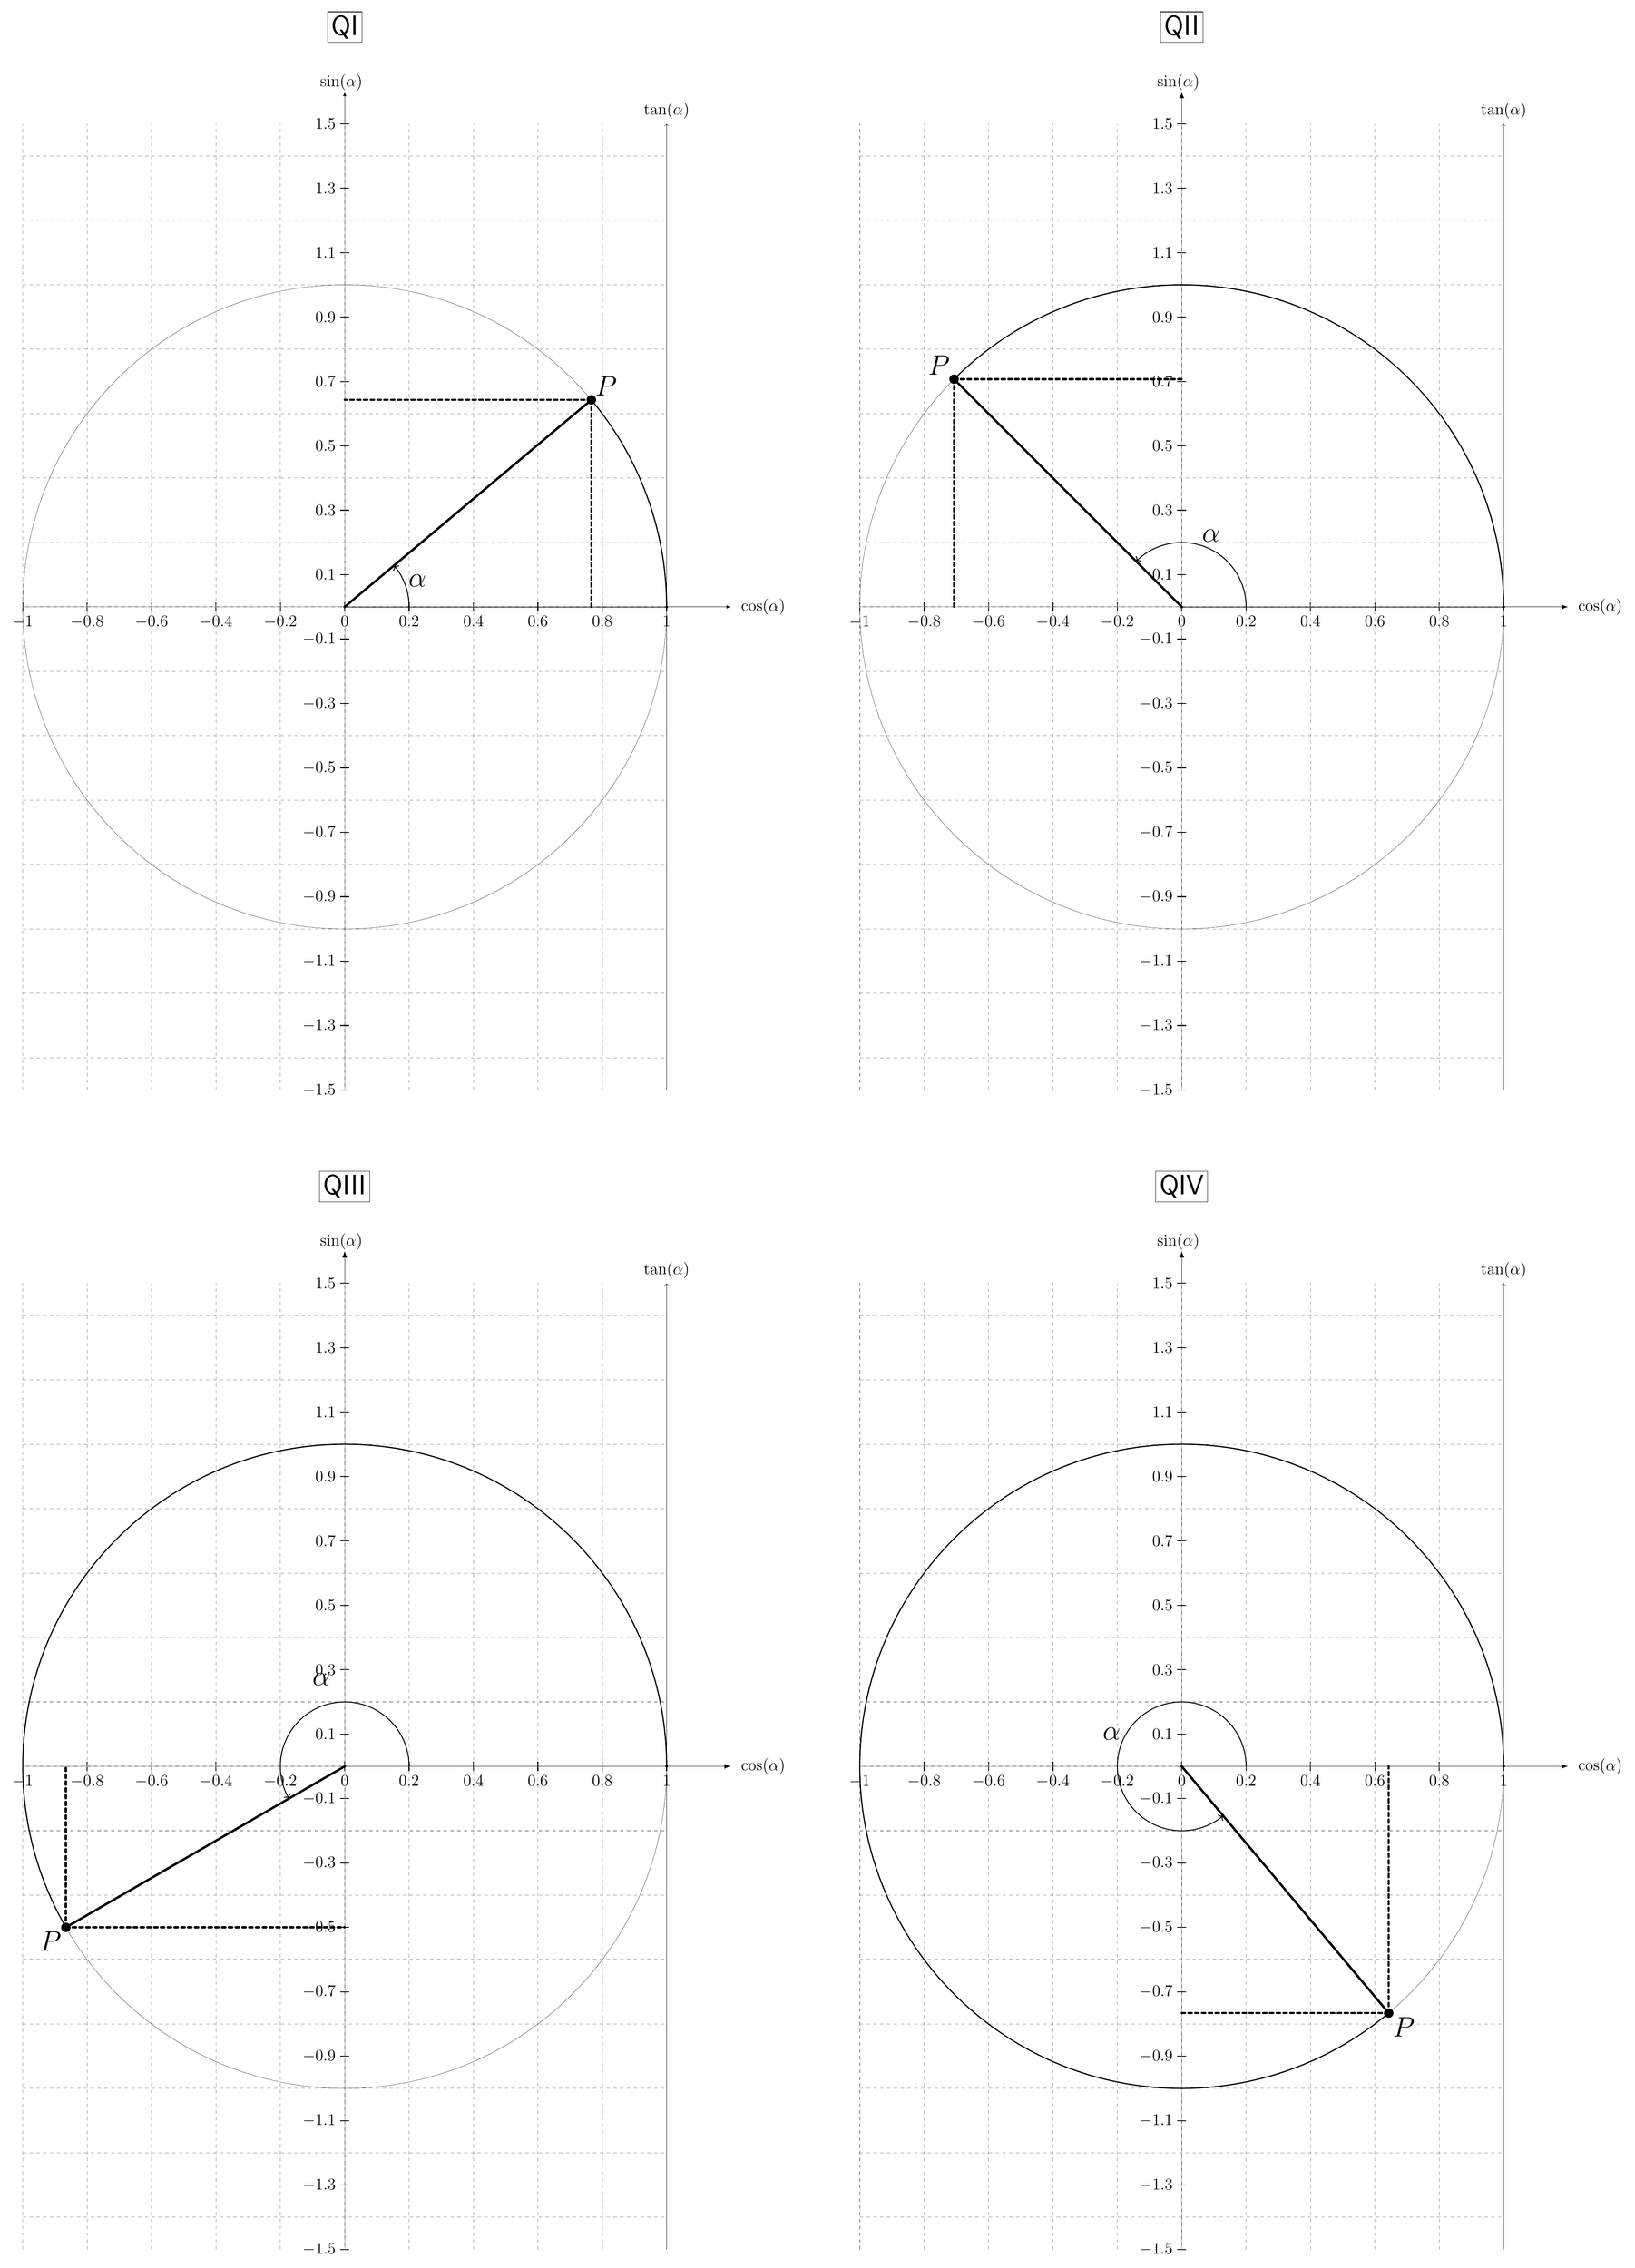
\begin{tikzpicture}[scale=2]
   \tkzInit[xmax=1.,ymax=1.5,xmin=-1. ,ymin=-1.5,xstep=0.2,ystep=0.2]
   \tkzDrawY[label=$\sin(\alpha)$, above, font=\Large]
   \tkzLabelY[node font=\Large]
   \tkzLabelX[node font=\Large]
   \tkzDrawX[label=$\cos(\alpha)$, right=8pt, font=\Large,right space=1]
   \tkzText[draw](0,1.8){\Huge QI}

   \begin{scope}[dashed]
     \tkzGrid
   \end{scope}
   \tkzDefPoints{0/0/O,1/0/A, 1/1/M,0/1/N}
   \tkzDrawCircle[color=black](O,A)
   \tkzDefPointBy[rotation= center O angle 40](A)
   \tkzGetPoint{P}
   \tkzDrawSegment(O,A)
   \tkzDrawSegment[line width=2pt](O,P)
   \tkzDrawArc[color=black,line width=1pt](O,A)(P)
   \tkzDrawPoints(A,P,O)
   \tkzDrawPoint[size=8](P)
   \tkzLabelPoint[above right](P){\Huge$P$}
   \tkzPicAngle["\Huge$\alpha$",draw=black,
->,angle eccentricity=1.2,
angle radius=2cm, thick](A,O,P)
\tkzInterLL(O,P)(A,M)
\tkzGetPoint{Q}

\tkzDefPointBy[projection= onto O--A](P)
\tkzGetPoint{PX}
\tkzDefPointBy[projection= onto O--N](P)
\tkzGetPoint{PY}
\tkzDrawSegments[dashed, line width=2pt](P,PX P,PY)
\tkzDefPoints{1/1.5/A,1/-1.5/B}
  \tkzDrawSegment[<-](A,B)
\tkzLabelSegment[line width=2pt, above, pos=0](A,B){\Large$\tan(\alpha)$}
\begin{scope}[xshift=13cm]
  \tkzDrawY[label=$\sin(\alpha)$, above, font=\Large]
  \tkzLabelY[node font=\Large]
  \tkzLabelX[node font=\Large]
  \tkzDrawX[label=$\cos(\alpha)$, right=8pt, font=\Large,right space=1]

  \begin{scope}[dashed]
    \tkzGrid
  \end{scope}
  \tkzDefPoints{0/0/O,1/0/A, 1/1/M,0/1/N}
  \tkzDrawCircle[color=black](O,A)
  \tkzDefPointBy[rotation= center O angle 135](A)
  \tkzGetPoint{P}
  \tkzDrawSegment(O,A)
  \tkzDrawSegment[line width=2pt](O,P)
  \tkzDrawArc[color=black,line width=1pt](O,A)(P)
  \tkzDrawPoints(A,P,O)
  \tkzDrawPoint[size=8](P)
  \tkzLabelPoint[above left](P){\Huge$P$}
  \tkzPicAngle["\Huge$\alpha$",draw=black,
->,angle eccentricity=1.2,
angle radius=2cm, thick](A,O,P)
\tkzInterLL(O,P)(A,M)
\tkzGetPoint{Q}
\tkzText[draw](0,1.8){\Huge QII}

\tkzDefPointBy[projection= onto O--A](P)
\tkzGetPoint{PX}
\tkzDefPointBy[projection= onto O--N](P)
\tkzGetPoint{PY}
\tkzDrawSegments[dashed, line width=2pt](P,PX P,PY)
\tkzDefPoints{1/1.5/A,1/-1.5/B}
  \tkzDrawSegment[<-](A,B)
\tkzLabelSegment[line width=2pt, above, pos=0](A,B){\Large$\tan(\alpha)$}
\end{scope}



\begin{scope}[yshift=-18cm]
  \tkzInit[xmax=1.,ymax=1.5,xmin=-1. ,ymin=-1.5,xstep=0.2,ystep=0.2]
  \tkzDrawY[label=$\sin(\alpha)$, above, font=\Large]
  \tkzLabelY[node font=\Large]
  \tkzLabelX[node font=\Large]
  \tkzDrawX[label=$\cos(\alpha)$, right=8pt, font=\Large,right space=1]

  \begin{scope}[dashed]
    \tkzGrid
  \end{scope}
  \tkzDefPoints{0/0/O,1/0/A, 1/1/M,0/1/N}
  \tkzDrawCircle[color=black](O,A)
  \tkzDefPointBy[rotation= center O angle 210](A)
  \tkzGetPoint{P}
  \tkzDrawSegment(O,A)
  \tkzDrawSegment[line width=2pt](O,P)
  \tkzDrawArc[color=black,line width=1pt](O,A)(P)
  \tkzDrawPoints(A,P,O)
  \tkzDrawPoint[size=8](P)
  \tkzLabelPoint[below left](P){\Huge$P$}
  \tkzPicAngle["\Huge$\alpha$",draw=black,
->,angle eccentricity=1.4,
angle radius=2cm, thick](A,O,P)
\tkzInterLL(O,P)(A,M)
\tkzGetPoint{Q}
\tkzText[draw](0,1.8){\Huge QIII}
\tkzDefPointBy[projection= onto O--A](P)
\tkzGetPoint{PX}
\tkzDefPointBy[projection= onto O--N](P)
\tkzGetPoint{PY}
\tkzDrawSegments[dashed, line width=2pt](P,PX P,PY)
\tkzDefPoints{1/1.5/A,1/-1.5/B}
  \tkzDrawSegment[<-](A,B)
\tkzLabelSegment[line width=2pt, above, pos=0](A,B){\Large$\tan(\alpha)$}
\begin{scope}[xshift=13cm]
 \tkzDrawY[label=$\sin(\alpha)$, above, font=\Large]
 \tkzLabelY[node font=\Large]
 \tkzLabelX[node font=\Large]
 \tkzDrawX[label=$\cos(\alpha)$, right=8pt, font=\Large,right space=1]
 \tkzText[draw](0,1.8){\Huge QIV}
 \begin{scope}[dashed]
   \tkzGrid
 \end{scope}
 \tkzDefPoints{0/0/O,1/0/A, 1/1/M,0/1/N}
 \tkzDrawCircle[color=black](O,A)
 \tkzDefPointBy[rotation= center O angle 310](A)
 \tkzGetPoint{P}
 \tkzDrawSegment(O,A)
 \tkzDrawSegment[line width=2pt](O,P)
 \tkzDrawArc[color=black,line width=1pt](O,A)(P)
 \tkzDrawPoints(A,P,O)
 \tkzDrawPoint[size=8](P)
 \tkzLabelPoint[below right](P){\Huge$P$}
 \tkzPicAngle["\Huge$\alpha$",draw=black,
->,angle eccentricity=1.2,
angle radius=2cm, thick](A,O,P)
\tkzInterLL(O,P)(A,M)
\tkzGetPoint{Q}

\tkzDefPointBy[projection= onto O--A](P)
\tkzGetPoint{PX}
\tkzDefPointBy[projection= onto O--N](P)
\tkzGetPoint{PY}
\tkzDrawSegments[dashed, line width=2pt](P,PX P,PY)
\tkzDefPoints{1/1.5/A,1/-1.5/B}
  \tkzDrawSegment[<-](A,B)
\tkzLabelSegment[line width=2pt, above, pos=0](A,B){\Large$\tan(\alpha)$}
\end{scope}
\end{scope}
\end{tikzpicture}
\end{document}
